\section{zadanie 4}
Zadanie polegało na napisanui funkcji która zinterpoluje zadaną funkcjię \(f(x)\) na zadanym przedziale \([a, b]\) za pomocą wielomianu interpolacyjnego stopnia n w postaci Newton oraz narysuje wielomian interpolacyjny i interpolowaną funkcjię. Do rysowania użyłem pakiety \textbf{PyPlot}.

Algorytm na wejściu dostaje funkcję \(f(x)\) zadaną jako anonimowa, \(a, b\) - krańce przedziału oraz \(n \in \mathbb{N} \) - stopień wielomianu interpolacyjnego.
Wynikiem działania funkcji jest obrazek zapisany do pliku na dysku.

\subsection{Opis działania: }
Pierwszym krokiem jest podzielenie przedziału \([a, b]\) na \(n\) równych podprzedziałów. Końce przedziału zapisujemy do tablicy argumentów \(x\), a wartości funkcji w tych miejscach do tablicy wartości funkcji \(y\). Następnie obliczamy ilorazy różnicowe dla 
uprzednio obliczonych argumentów i wartości \(yN\).\\
Kolejnym krokiem jest zwiększenie 'rozdzielczości', wykonujemy to przez przemnożenie stopnia wielomian przez stałą \(factor\). Tak jak poprzednio obliczamy nowe argumenty oraz wartości funkcji jednak dodatkowo na podstawie poprzednio policzonych argumentów i wartości korzystamy z funkcji \textbf{warNewton} aby policzyć wierzchołki wielomianu interpolacyjnego.\\
końcowym etapem jest wykorzystanie pakietu \textbf{PyPlot} do naniesienia danych na wykresy oraz zapisanie obrazków.

\subsection{Dla przykładowych funkcji: }

\begin{figure}[ht]
  \begin{subfigure}{0.5\textwidth}
    \centering
    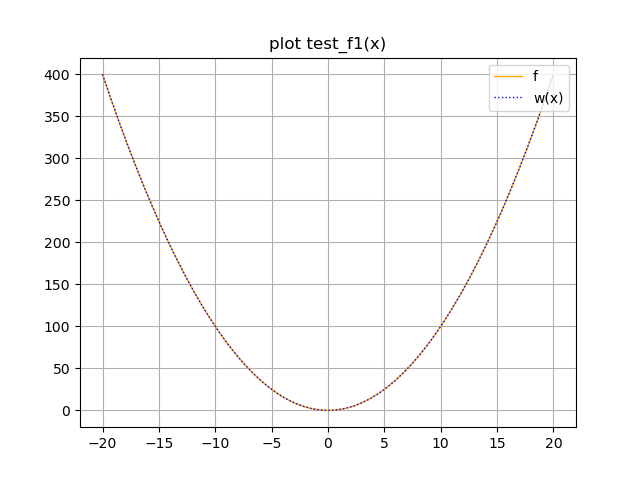
\includegraphics[width=\linewidth]{plot_test_f1(x)_10.png}
    \caption{\(f(x) = x^2, n = 10\)}
  \end{subfigure}
  \begin{subfigure}{0.5\textwidth}
    \centering
    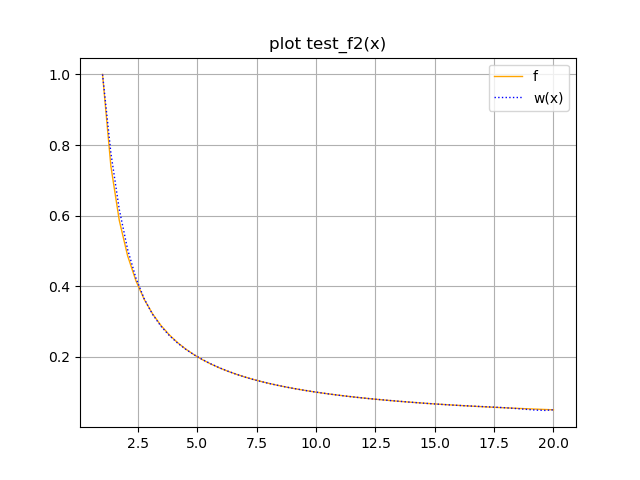
\includegraphics[width=\linewidth]{plot_test_f2(x)_10.png}
    \caption{\(f(x) = 1/x, n = 10\)}
  \end{subfigure}

  \begin{subfigure}{0.5\textwidth}
    \centering
    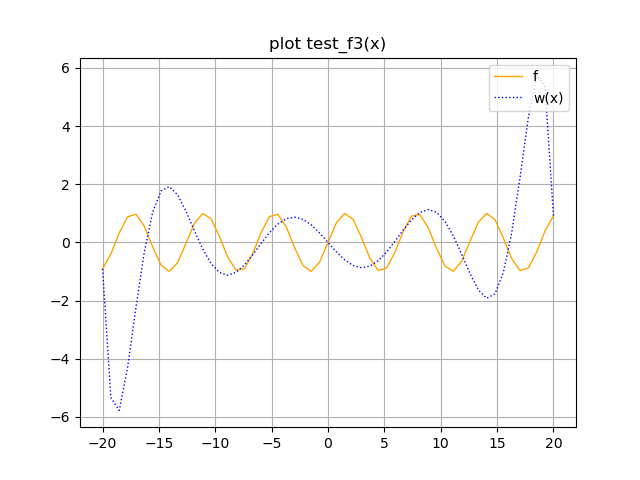
\includegraphics[width=\linewidth]{plot_test_f3(x)_10.png}
    \caption{\(f(x) = \sin(x), n = 10\)}
  \end{subfigure}
  \begin{subfigure}{0.5\textwidth}
    \centering
    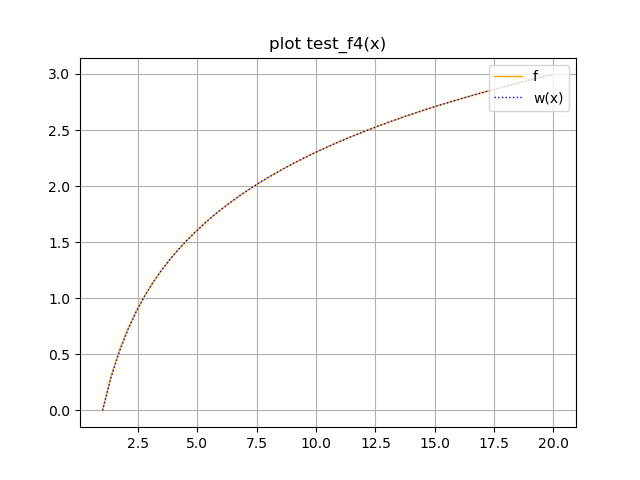
\includegraphics[width=\linewidth]{plot_test_f4(x)_10.png}
    \caption{\(f(x) = \log(x), n = 10\)}
  \end{subfigure}
\end{figure}